\documentclass[a4paper,reqno]{amsart}
\usepackage{amssymb}
\usepackage{color}
\usepackage{tikz}
\usetikzlibrary{patterns}

\begin{document}

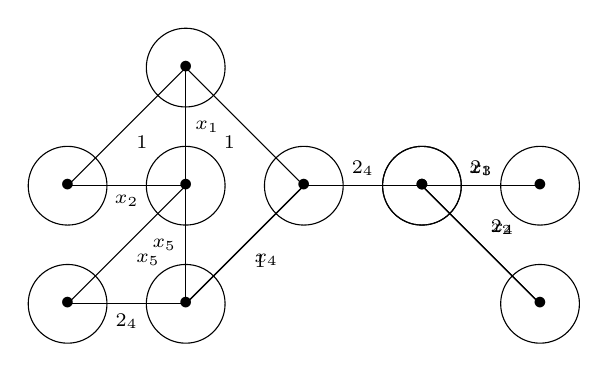
\begin{tikzpicture}[xscale=.5,yscale=.5]
\draw (0,0) -- node[auto] {$\scriptstyle{2_4}$} (3,0);
\draw (0,0) -- node[auto] {$\scriptstyle{1}$} (-3,3);
\draw (0,0) -- node[auto] {$\scriptstyle{1}$} (-3,-3);
\draw (3,0) -- node[auto] {$\scriptstyle{2_1}$} (6,0);
\draw (0,0) -- node[auto] {$\scriptstyle{x_4}$} (-3,-3);
\draw (3,0) -- node[auto] {$\scriptstyle{2_2}$} (6,-3);
\draw (-3,3) -- node[auto] {$\scriptstyle{1}$} (-6,0);
\draw (-3,-3) -- node[auto] {$\scriptstyle{2_4}$} (-6,-3);
\draw (-3,3) -- node[auto] {$\scriptstyle{x_1}$} (-3,0);
\draw (-3,-3) -- node[auto] {$\scriptstyle{x_5}$} (-3,0);
\draw (3,0) -- node[auto] {$\scriptstyle{x_3}$} (6,0);
\draw (-3,0) -- node[auto] {$\scriptstyle{x_2}$} (-6,0);
\draw (-3,0) -- node[auto] {$\scriptstyle{x_5}$} (-6,-3);
\draw (3,0) -- node[auto] {$\scriptstyle{x_4}$} (6,-3);
\draw (0,0) circle [radius=1];
\node at (0,0) {$\bullet$};
\draw (-3,0) circle [radius=1];
\node at (-3,0) {$\bullet$};
\draw (3,0) circle [radius=1];
\node at (3,0) {$\bullet$};
\draw (-3,3) circle [radius=1];
\node at (-3,3) {$\bullet$};
\draw (-3,-3) circle [radius=1];
\node at (-3,-3) {$\bullet$};
\draw (3,0) circle [radius=1];
\node at (3,0) {$\bullet$};
\draw (6,0) circle [radius=1];
\node at (6,0) {$\bullet$};
\draw (6,-3) circle [radius=1];
\node at (6,-3) {$\bullet$};
\draw (-6,0) circle [radius=1];
\node at (-6,0) {$\bullet$};
\draw (-6,-3) circle [radius=1];
\node at (-6,-3) {$\bullet$};

\end{tikzpicture}
\hspace{1cm}
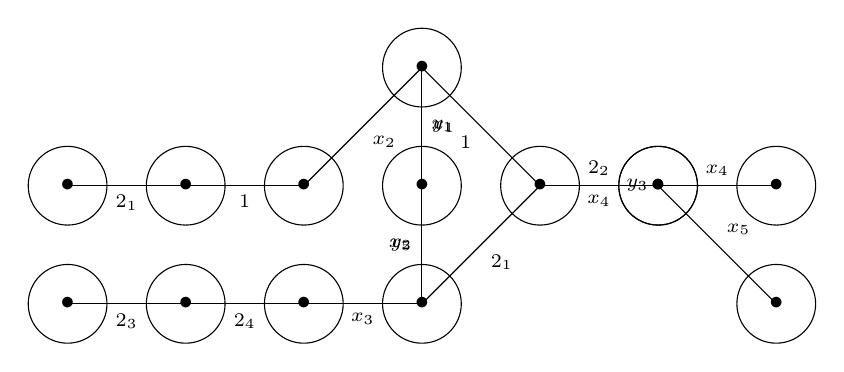
\begin{tikzpicture}[xscale=.5,yscale=.5]
\draw (0,0) -- node[auto] {$\scriptstyle{1}$} (-3,3);
\draw (0,0) -- node[auto] {$\scriptstyle{2_1}$} (-3,-3);
\draw (0,0) -- node[auto] {$\scriptstyle{2_2}$} (3,0);
\draw (-3,3) -- node[auto] {$\scriptstyle{x_1}$} (-3,0);
\draw (-3,-3) -- node[auto] {$\scriptstyle{x_5}$} (-3,0);
\draw (3,0) -- node[auto] {$\scriptstyle{x_4}$} (0,0);
\draw (-3,3) -- node[auto] {$\scriptstyle{x_2}$} (-6,0);
\draw (-3,-3) -- node[auto] {$\scriptstyle{x_3}$} (-6,-3);
\draw (3,0) -- node[auto] {$\scriptstyle{x_4}$} (6,0);
\draw (3,0) -- node[auto] {$\scriptstyle{x_5}$} (6,-3);
\draw (-3,3) -- node[auto] {$\scriptstyle{y_1}$} (-3,0);
\draw (-3,-3) -- node[auto] {$\scriptstyle{y_2}$} (-3,0);
\draw (3,0) -- node[auto] {$\scriptstyle{y_3}$} (3,0);
\draw (-6,0) -- node[auto] {$\scriptstyle{1}$} (-9,0);
\draw (-6,-3) -- node[auto] {$\scriptstyle{2_4}$} (-9,-3);
\draw (-3,0) circle [radius=1];
\node at (-3,0) {$\bullet$};
\draw (0,0) circle [radius=1];
\node at (0,0) {$\bullet$};
\draw (3,0) circle [radius=1];
\node at (3,0) {$\bullet$};
\draw (-3,3) circle [radius=1];
\node at (-3,3) {$\bullet$};
\draw (-3,-3) circle [radius=1];
\node at (-3,-3) {$\bullet$};
\draw (3,0) circle [radius=1];
\node at (3,0) {$\bullet$};
\draw (6,0) circle [radius=1];
\node at (6,0) {$\bullet$};
\draw (6,-3) circle [radius=1];
\node at (6,-3) {$\bullet$};
\draw (-6,0) circle [radius=1];
\node at (-6,0) {$\bullet$};
\draw (-6,-3) circle [radius=1];
\node at (-6,-3) {$\bullet$};
\draw (-9,0) circle [radius=1];
\node at (-9,0) {$\bullet$};
\draw (-9,-3) circle [radius=1];
\node at (-9,-3) {$\bullet$};
\draw (-9,0) -- node[auto] {$\scriptstyle{2_1}$} (-12,0);
\draw (-9,-3) -- node[auto] {$\scriptstyle{2_3}$} (-12,-3);
\draw (-12,0) circle [radius=1];
\node at (-12,0) {$\bullet$};
\draw (-12,-3) circle [radius=1];
\node at (-12,-3) {$\bullet$};

\end{tikzpicture}
\end{document}